\section{Laboratory work implementation}

\subsection{Tasks and Points}

\begin{enumerate}
\item Inițializarea unui nou repozitoriu
\item Configurarea VC
\item Crearea branch-urilor (cel puțin 2)
\item Commit pe ambele branch-uri (cel puțin 1 commit per branch)
\item Setarea unui branch sa urmărească un remote origin pe care se poate să faci push (GitHub)
\item Resetarea unui branch pe commit-ul anterior
\item Folosirea fișierului .gitignore
\item Merge dintre 2 branch-uri
\item Rezolvarea confilectelor a 2 branch-uri
\item Folosirea tag-urilor pentru marcarea schimbarilor semnificative precum release
\end{enumerate}

\subsection{Analiza lucrarii de laborator}

\begin{enumerate}

\item Primul pas a fost inițializarea unui nou repozitoriu

\begin{minipage}{\linewidth}
	\centering
	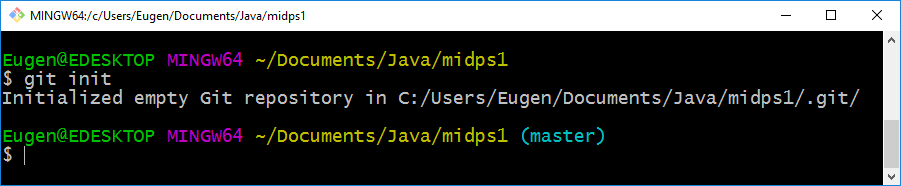
\includegraphics[width=17cm]{01init}
	\captionof{figure}{Inițializarea repozitoriului}
\end{minipage}
\break

\item Pentru a defini autorul versiunilor am folosit comanda \textbf{git config}

\begin{minipage}{\linewidth}
	\centering
	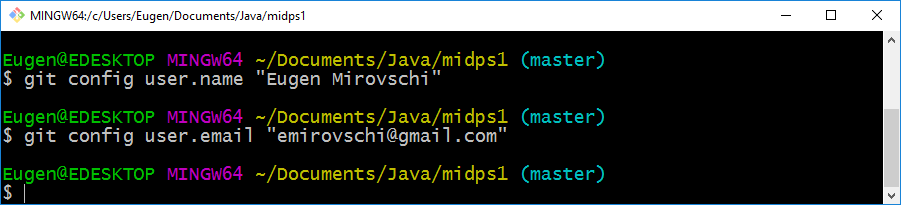
\includegraphics[width=17cm]{02config}
	\captionof{figure}{Configurarea repozitoriului}
\end{minipage}
\break

\item Branch-ul master a fost create utilizând comanda \textbf{git checkout -b master} după care a fost adăugat un fișier nou care este inclus în primul commit

\begin{minipage}{\linewidth}
	\centering
	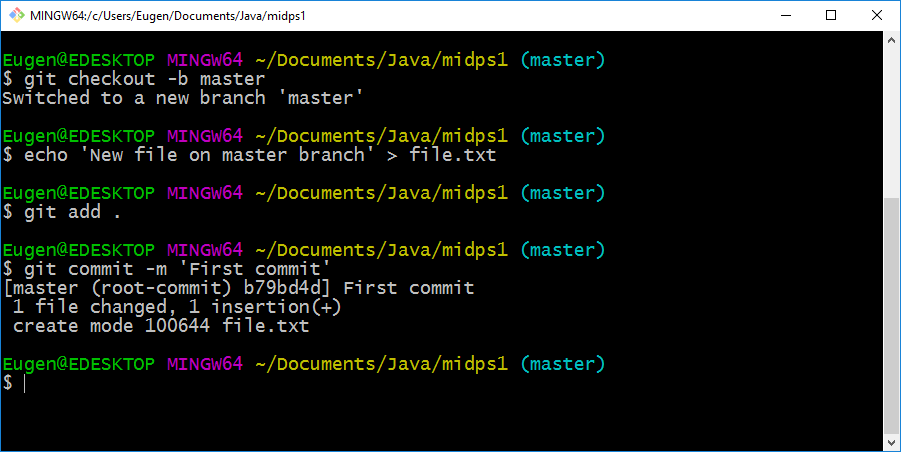
\includegraphics[width=17cm]{03masterBranch}
	\captionof{figure}{Crearea master branch}
\end{minipage}
\break

\item Branch-ul develop a fost creat similar ca și master însă acesta are automat ca parent primul commit din master.

\begin{minipage}{\linewidth}
	\centering
	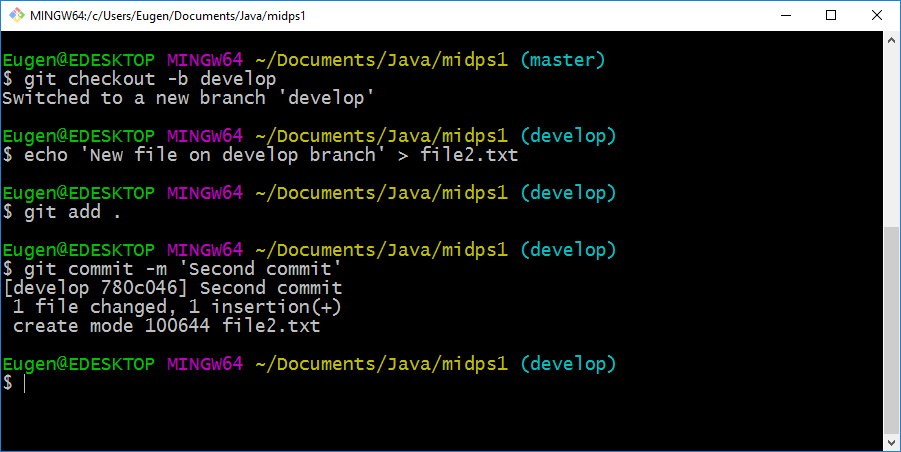
\includegraphics[width=17cm]{04developBranch}
	\captionof{figure}{Crearea develop branch}
\end{minipage}
\break

\item Pentru a adăuga un remote, inițial am creat un repozitoriu nou în GitHub după care am rulat comanda de adaugare a referinței în repozitoriul local \textbf{git remote add}. După aceasta am mutat toate schimbarile pe origin folosind \textbf{git push}. Repozitoriul folosind în acest caz este \url{https://github.com/emirovschi/MIDPS-1}.

\begin{minipage}{\linewidth}
	\centering
	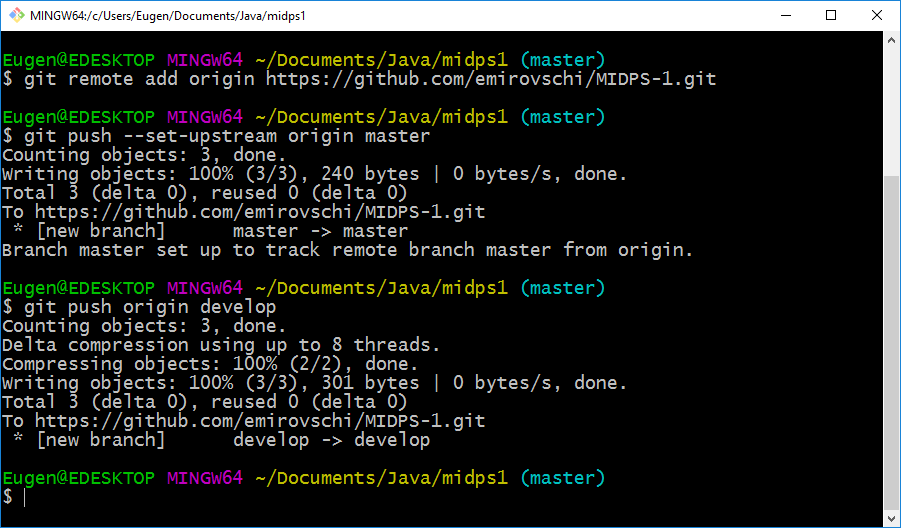
\includegraphics[width=17cm]{05remote}
	\captionof{figure}{Adăugare remote}
\end{minipage}
\break

\item Pentru a reseta branch-ul curent la commitul anterior am folosit commanda \textbf{git reset HEAD~}.

\begin{minipage}{\linewidth}
	\centering
	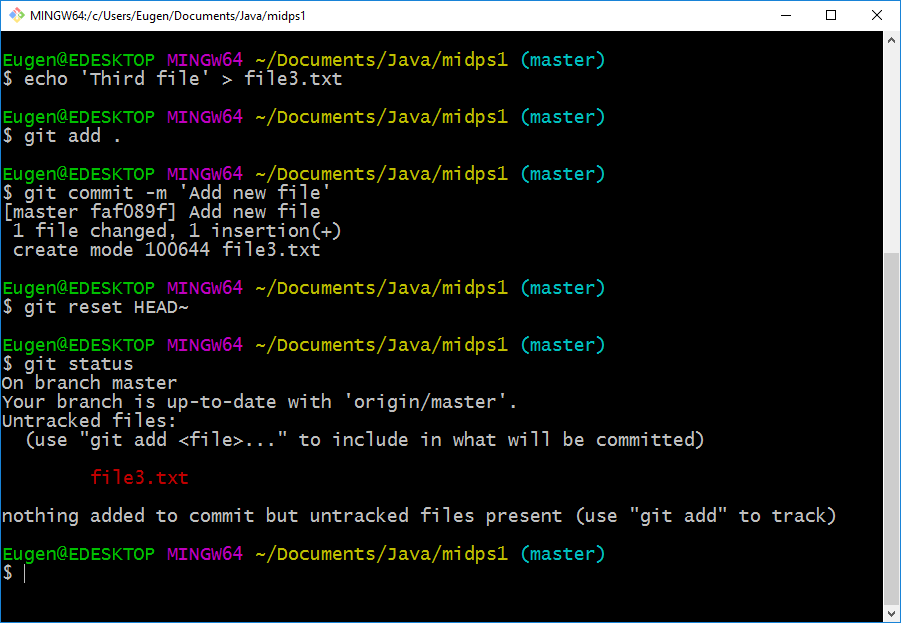
\includegraphics[width=17cm]{06reset}
	\captionof{figure}{Resetarea ultimului commit}
\end{minipage}
\break

\item Fișierul \textit{.gitignore} permite excluderea anumitor fișiere în dependență de denumirea acestora. În exemplul dat am exclus fișierul creat în pasul anterior.

\begin{minipage}{\linewidth}
	\centering
	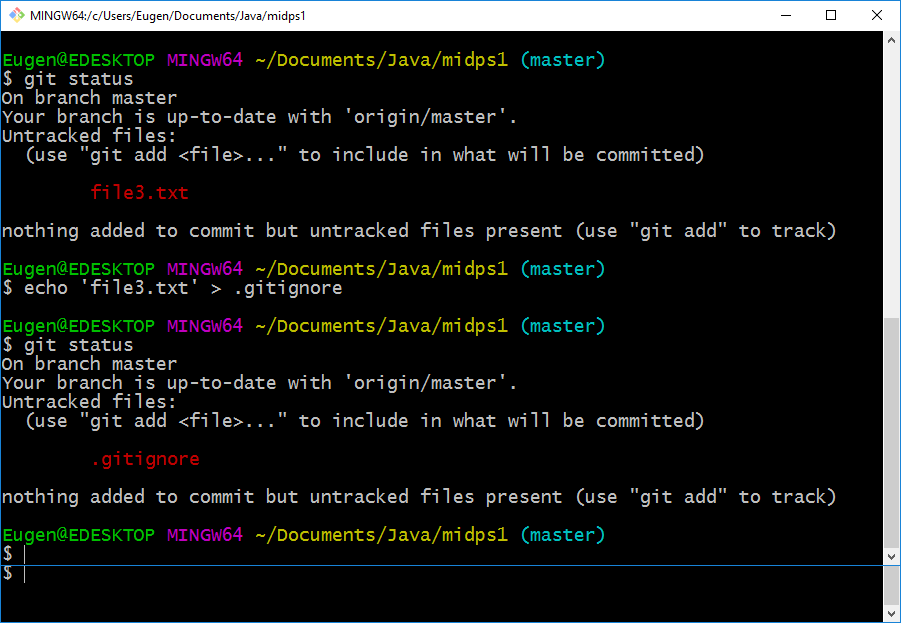
\includegraphics[width=17cm]{07ignore}
	\captionof{figure}{Adăugarea unui fișier în .gitignore}
\end{minipage}
\break

\item Merge între branch-uri se face utilizând comanda \textbf{git merge}. În acest exemplu am facut merge la develop branch în master

\begin{minipage}{\linewidth}
	\centering
	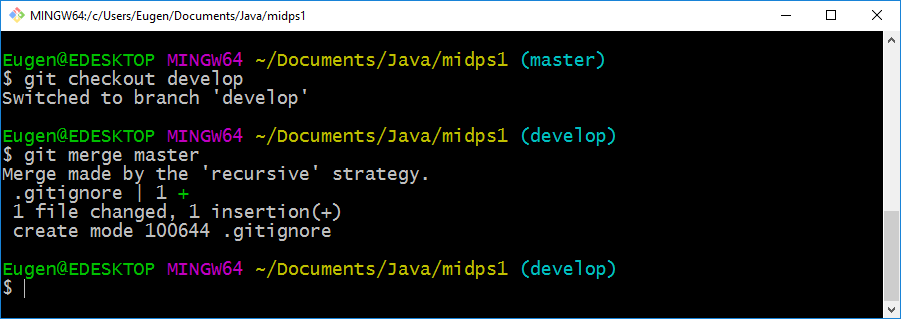
\includegraphics[width=17cm]{08merge}
	\captionof{figure}{Branch merge}
\end{minipage}
\break

\item În caz că o linie dintr-un fișier a fost redactată pe ambele branch-uri, atunci posibil să conflicteze în procesul de merge a branch-urilor.

\begin{minipage}{\linewidth}
	\centering
	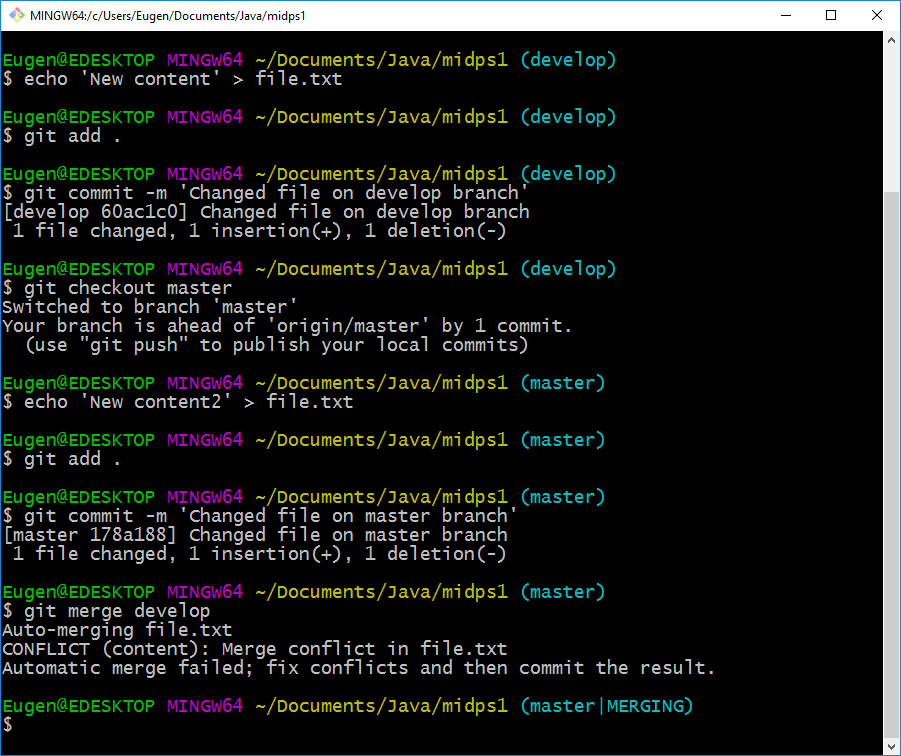
\includegraphics[width=17cm]{09conflict}
	\captionof{figure}{Simularea unui conflict}
\end{minipage}
\break

\item Soluționarea unui conflict poate fi efectuată prin mai multe metode: redactarea manuală, utilizarea unui instrument de comparare sau folosirea uneia din versiuni. În acest caz am forțat folosirea versiunii curente.

\begin{minipage}{\linewidth}
	\centering
	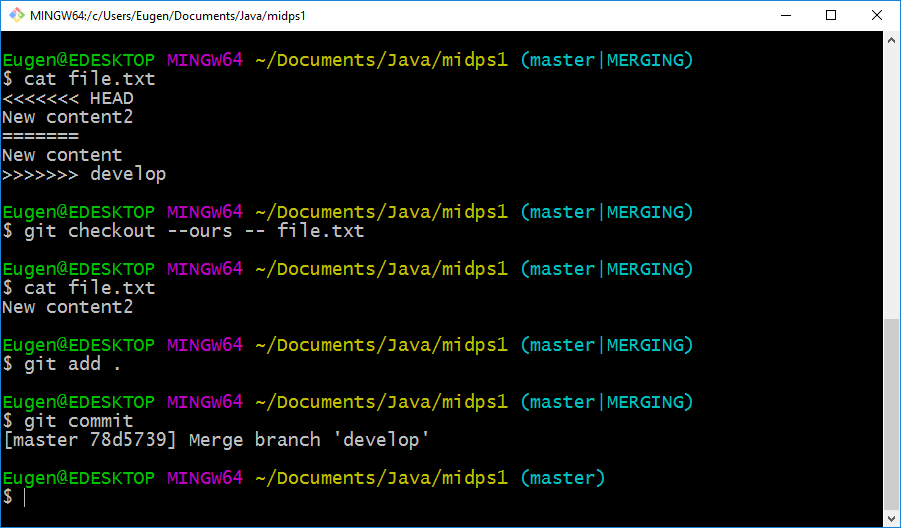
\includegraphics[width=17cm]{10resolve}
	\captionof{figure}{Soluționarea unui conflict}
\end{minipage}
\break

\item Crearea unui tag este efectuată utilizând comanda \textbf{git tag}. Aceasta atașează tag-ul nou la commit-ul current.

\begin{minipage}{\linewidth}
	\centering
	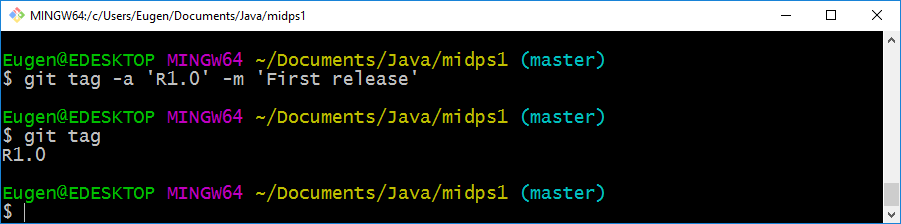
\includegraphics[width=17cm]{11tag}
	\captionof{figure}{Crearea unui tag}
\end{minipage}
\break

\end{enumerate}


